\section{Experiment and Evaluation}
\label{sec:results}

We evaluate the performance based on the data collected from 24 subjects, who are mainly graduate students between 25 to 35-year old. We choose a 19-paragraph, 830-word article from \textit{New York Times} and then ask each subject to write the whole article \jingap{once} | in front of a Leap Motion sensor from time to time over a period of 7 months. The word length varies from 1 to 14 characters. 

Writing in the air is prone to cause arm fatigue~\cite{Consumed_Endurance_fatigue_CHI_2014}. Since
the least physically demanding position keeps the upper-arm
at rest~\cite{Cockburn_AirPointing_2011HCS}, we let the subjects lay their elbows on a table
to rest their upper-arms, and bend their elbows to further
reduce fatigue. The larger the angle between the table and
the subjects' forearms, the less fatigue they experienced. In
addition, we adjusted the position of the Leap Motion to make
the users' hand visible.
Specifically, we place the Leap Motion sensor facing up at the right side of the laptop computer, or between the computer monitor and the keyboard of a desktop computer as shown in~\figref{fig:leap}. 

We first collect normal data for 24 subjects independently, i.e., each subject writes the article without observing any other subjects.  \jingap{We use the first few paragraphs for enrollment and the rest for testing without cross validation. We get 3256 samples in total, and include 10 words in a sample on average. Among them, 720 samples are for training, and others are used for testing. }
\jingap{Then, we collect data from 7 subjects who act as observing attackers. In total, 84 attack samples are collected.}  



\begin{table*}[!btph]
%\scriptsize
\centering
\vspace{-0mm}
  \caption {\jing{The EER of one victim subject attacked by $23$ Non-Observing insiders with various parameters. The results are averaged with 24 victim subjects. We varied one parameter at a time and use the following default parameters: one sample contains no more than 2,000 frames; each experiment uses 30 samples per subject for training and the rest for testing; each stroke segment  contains 12 frames; each experiment has a vocabulary size of $K=200$.}  
\label{tab: AllRes}}
\begin{tabular}{|r|cccccc|} \hline
%\multicolumn{7}{|c|}{{   }} \\
%\multicolumn{7}{|c|}{{ $wps$; }} \\
%\multicolumn{7}{|c|}{{  }} \\ \hline
Sample Length ($\#$Frames) & 500   & 1,000  & \textbf{2,000}    & 3,000 & 4,000 &5,000 \\
Words per Sample \textbf{$wps$} & 2.5  	& 5   & \textbf{10}     & 15 & 20  &25 \\	
Writing Time per Sample	& 4.4s   	& 8.8s   & \textbf{17.5s}     & 26.3s  & 35.1s  &43.9s \\
\jing{Writing Time for Training (Total)}	& 2.2min   	& 4.4min & \textbf{8.7min}     & 13.5min  & 17.5min  &21.9min \\
 \textbf{EER}  & $6.79\%$ & $3.11\%$ & \textbf{$1.18\%$} & $1.01\%$ & $0.38\%$  & $0.32\%$  \\ \hline  \hline

%\multicolumn{7}{|c|}{{ }} \\ \hline
No. of Training Samples  	& 10  		& 20  		& \textbf{30}     		& 40  			& 50 		&  \\
 \textbf{EER}  & $2.35\%$ & $1.63\%$ & \textbf{$1.18\%$} 	& $ 0.98\%$ 	& $0.91\%$ &  \\ \hline \hline

%\multicolumn{7}{|c|}{{$L_c$}} \\ \hline
Stroke Segment Length  ($\#$Frames)     	& 8    			& \textbf{12}    	 & \jing{16}  			&20    &  & \\
 \textbf{EER}  	& $2.48\%$  	& \textbf{$1.18\%$} & \jing{$1.34\%$} 	&$1.65\%$  &  &  \\   \hline  \hline
%
%\multicolumn{7}{c}{\textbf{Component Overlapping percentage}} \\ \hline
%  \textbf{\% Overlapping}      & None        & Half  	& \textbf{Two-third}  &  &   &\\
%  \textbf{Accuracy} 	   & $96.74\%$   & $97.15$ 	& \textbf{$97.42\%$}  &  & 	 &  \\  \hline  \hline

%\multicolumn{7}{|c|}{{ }} \\ \hline
Vocabulary Size  \textbf{$K$}   	& 50   		 & 100    	  & \textbf{200}       & 400 	   &    &   \\
  \textbf{EER} & $5.39\% $ & $3.54\%$  & \textbf{$1.18\%$} & $0.87\%$ &    &   \\  \hline \hline  
  
Style-level Feature    	& Histogram   		 & Co-occurrence    	  & Combined        &  	   &    &   \\
      &    		 & Matrix    	  & Both       &  	   &    &   \\
  \textbf{EER} & $5.45\% $ & $1.18\%$  & \textbf{$2.01\%$} &   &    &   \\  \hline   
  %\hline
  
\end{tabular}
\vspace{-0mm}
\end{table*}


% (details are described in Section~\ref{subsec:rejecRes}). 

%%==================================================================================================




%For evaluation, we compute the following metrics to examine the performance under attacks:
%\begin{inlinenum}
%\item $tp$, the number of true positives,
%\item $tn$, the number of true negatives, 
%\item $fp$, the number of false positives, and 
%\item $fn$, the number of false negatives.
%\end{inlinenum} 
%Given that the training data samples can be randomly selected, we can conduct multiple rounds of experiments and calculate these four metrics at each round. This way, we can compute the true positive rate (TPR), and the false positive rate (FPR) as
%
%$$ TPR = \frac{\sum_{i=1}^m tp_i}{\sum_{i=1}^m tp_i+\sum_{i=1}^m fn_i},\quad
% FPR = \frac{\sum_{i=1}^m fp_i}{\sum_{i=1}^m fp_i+\sum_{i=1}^m tn_i}.$$
%where $i=1,2,\cdots, m$ indicates the $i$-th round of experiments. We plot the standard ROC curves to quantitatively evaluate the performance of rejecting a observing attacker. The \textbf{ROC curve} stands for the receiver operating characteristic curve and is a plot of the TPR against FPR by varying the threshold of the binary SVM classifiers. The closer the curve to the top-left corner $(0, 1)$, the better the authentication performance. 

\subsection{Results on CR Authentication}

\subsubsection{Evaluation Metrics}

\indent In the experiment, we verify whether a testing sample is written by a given legitimate user or not. The output is binary -- either `yes' or `no'.
 %As discussed in~\secref{sec:classification}, we train a binary SVM classifier for each legitimate subject and use samples from attackers to test the performance of the system. Given the binary SVM output, we apply a threshold to determine if the testing sample belongs to this user. 
 %\jing{We use receiver operating characteristic (ROC) curves and an equal error rate (EER) for evaluation. A ROC curve is generated by plotting the true positive rate (TPR) against the false positive rate (FPR) at various thresholds. The closer the curve to the top-left corner $(0, 1)$, the better the authentication performance. 
% In attack scenarios, we verify whether a testing sample is written by one of the legitimate users or not. The output is binary -- either `yes' or `no'.
 As discussed in~\secref{sec:classification}, we train a binary SVM classifier for each legitimate subject and use samples from attackers and each legitimate user to test the performance of the system. Given the binary SVM output, we apply a threshold to determine if the testing sample belongs to this user. 
 %One time authentication performance is evaluated for each subject separately, since they are trying to mimic a specific victim. We apply a threshold to determine if the skilled alien sample can passed the authentication. %
For evaluation, we compute the following metrics to examine the performance under attacks:
%\vspace{-2mm}
\begin{inlinenum}
\item $tp$, the number of true positives,
\item $tn$, the number of true negatives, 
\item $fp$, the number of false positives, and 
\item $fn$, the number of false negatives.
%\end{itemize}
\end{inlinenum} 


Given that the training data samples can be randomly selected, we can conduct multiple rounds of experiments and calculate these four metrics at each round. This way, we can compute the true positive rate (TPR), and the false positive rate (FPR) as
\begin{align}
\nonumber TPR &= \frac{\sum_{i=1}^m tp_i}{\sum_{i=1}^m tp_i+\sum_{i=1}^m fn_i}, \\
\nonumber FPR &= \frac{\sum_{i=1}^m fp_i}{\sum_{i=1}^m fp_i+\sum_{i=1}^m tn_i}.
\end{align}
where $i=1,2,\cdots, m$ indicates the $i$-th round of experiments. We plot the standard ROC curves to quantitatively evaluate the performance of rejecting a skilled attacker. The \textbf{ROC curve} stands for the receiver operating characteristic curve and is a plot of the TPR against FPR by varying the threshold of the binary SVM classifiers. The closer the curve to the top-left corner $(0, 1)$, the better the authentication performance. An \textbf{Equal Error Rate (EER)} is the one where the FPR equals to the false negative rate (FNR). The smaller the EER, the better the performance.



%\textbf{Histogram vs. Co-occurrence Matrix.} We conduct an experiment to justify choosing transition co-occurrence matrix of components as the sample features. In this experiment, we directly use the histogram of the individual (quantized) component features (i.e., the histogram of the component indices), the identification accuracy is only $83.4\%$, which is much lower than $97.4\%$ that uses the proposed sample features (i.e., co-occurrence matrix).  In addition, we combine two features (both histogram and co-occurrence matrix), but the accuracy (i.e., $96.0\%$) is not as high as the ones using only co-occurrence matrix. Therefore, we conclude that the component-transition statistics can better represent the handwriting style.
%
% 




 
\subsubsection{Results for Non-Observing Attackers}
\label{sec:para}

\begin{figure}[!b]
\centering
\vspace{-6mm}
{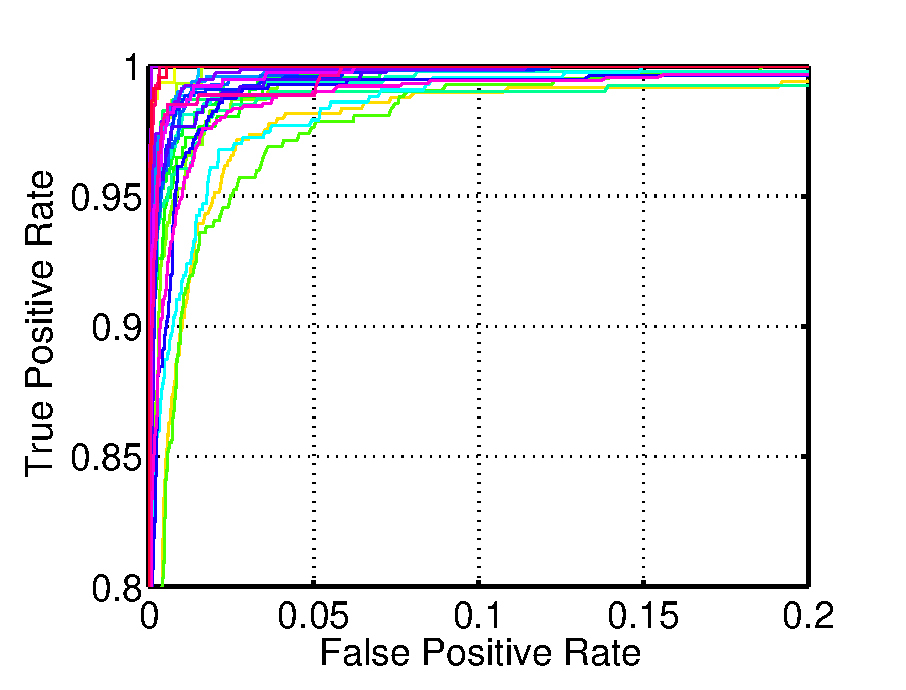
\includegraphics[width=.8\columnwidth]{./Graphic/roc/fig_11_24random.eps}}
%{\includegraphics[width=.8\columnwidth]{./Graphic/roc/ROC_24victim_random.eps}}
%(a) &(b)
\vspace{-3mm}
\caption{Performance of all $24$ subjects under Non-Observing attacks from insiders (samples from the rest of 23 subjects) presents by ROC curves. Each colored curve corresponds to the ROC of one subject.}
%\vspace{-1mm}
\label{fig:random}
%\vspace{-1mm}
\end{figure}


\begin{figure}[!b]
\centering
\vspace{-6mm}
%{\includegraphics[width=.8\columnwidth]{./Graphic/roc/leaveOneOut_imposter_roc.eps}}
{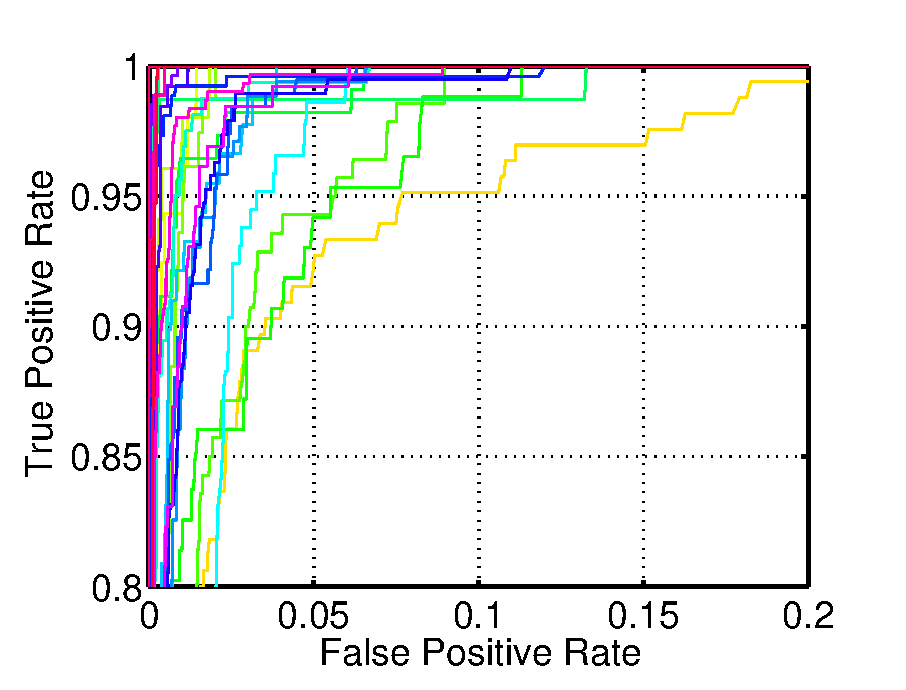
\includegraphics[width=.8\columnwidth]{./Graphic/roc/fig_12_24randomImpostor.eps}} \\
%(a) &(b)
\vspace{-3mm}
\caption{\jingap{Performance of all 24 subjects rejecting impostors presents by ROC curves. Each colored curve corresponds to the ROC of one subject.}}
%\vspace{-1mm}}
\label{fig:randomAliens}
%\vspace{-1mm}
\end{figure}

 


\textbf{Non-observing insiders.} 
To evaluate the performance under non-observing insiders, 
%we set the experiment as each subject is considered as a victim and the remaining $23$ subjects are considered as attackers. 
we utilize data from 24 subjects, train twenty-four classifiers with the training set and test them with the remaining data. For each classifier, one subject act as the victim (positive samples) and the rest 23 subjects act as attackers (negative  samples). Note that the data from the 24 subjects that are used for training are not used for testing.




\begin{figure*}[!b]
\centering
\vspace{-3mm}
\begin{tabular}{cc}
\subfigure
{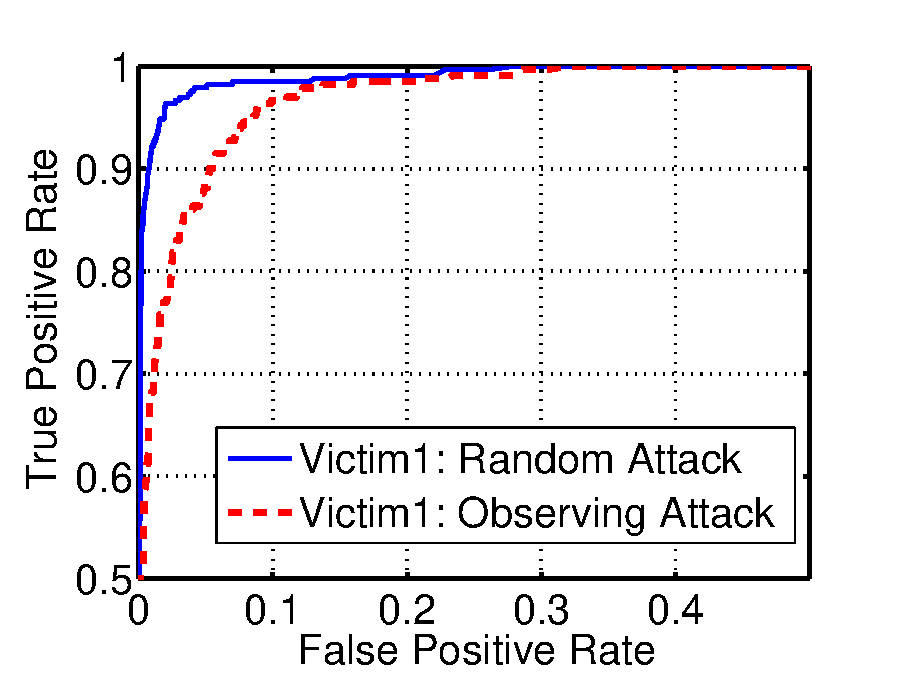
\includegraphics[width=.65\columnwidth]{./Graphic/roc/Roc_4victims_0_5_1st.eps}\vspace{-2mm}}
\subfigure
& {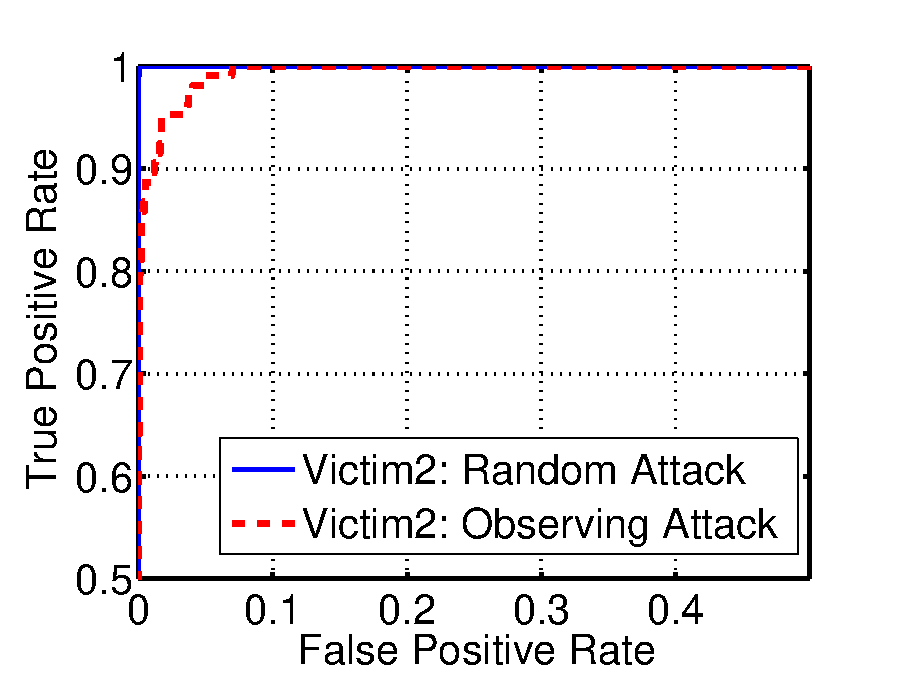
\includegraphics[width=.65\columnwidth]{./Graphic/roc/Roc_4victims_0_5_2st.eps}\vspace{-2mm}} \\ 

\subfigure
{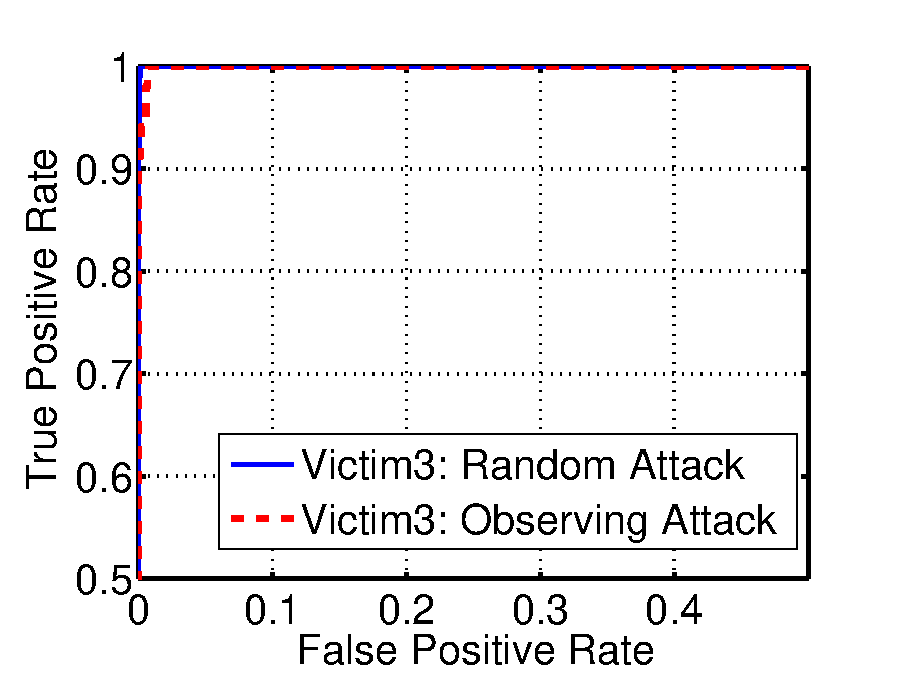
\includegraphics[width=.65\columnwidth]{./Graphic/roc/Roc_4victims_0_5_3st.eps}} 
\subfigure
& {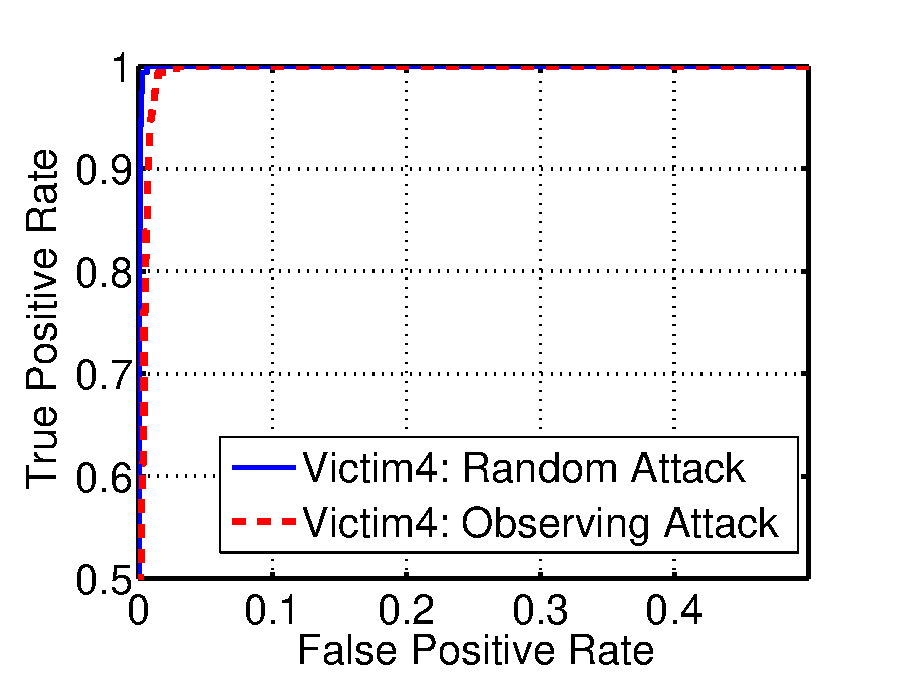
\includegraphics[width=.65\columnwidth]{./Graphic/roc/Roc_4victims_0_5_4st.eps}} 
\end{tabular}
\vspace{-0mm}
\caption{{Authentication performance of the victims under observing attacks presents by ROC curves. }}\label{fig:ROC_attack}
%\end{minipage}
\vspace{-0mm}
\end{figure*}


 Results are based on default parameters (one sample contains no more than $2,000$ frames; a training set contains $30$ samples per subject, the rests are for testing; each stroke segment contains $12$ frames; the vocabulary size equals to $200$). Figure~\ref{fig:random} shows the results where each ROC curve represents one subject. We observe that for almost all the subjects, the performance under Non-Observing attacks are close to ideal, near $100\%$ TPR, 0 FPR. \jingap{The worst cases are mainly caused by some of their samples that show similar styles (i.e., represented by similar co-occurrence matrices) to a few other subjects.}  We further calculated an average EER of 1.18\% among the $24$ subjects.

%The ROC curves are used for evaluation scenarios where an attacker may be an insider. 
%We also consider the impostor scenarios, i.e., an attacker does not belong to any of the enrolled subjects. \CiT rejects a testing sample as an impostor if the sample is rejected by all the binary SVM classifiers. To evaluate the performance of impostor rejection, we use rejection rate:
%$$ Rejection \;  Rate (R) = \frac{ \# Rejected \; Impostors}{\# Impostors}. $$ 
%The higher the value of $R$, the securer the \CiT system  in excluding impostors.  


\noindent 
\textit{\texttt{Varying Parameters.}}
%
%We vary parameters in this experiment to select default parameters which are used in the rest of the experiments. We choose the sample length from 500 to 4000 frames, and achieve an EER of 6.79\% ($L_s=500$), 3.12\% ($L_s=1000$), 1.18\% ($L_s=2000$), 0.38\% ($L_s=4000$). 
%Based on the trade-off between the computing overhead and the performance, we select the default sample length to be $2,000$ frames, and create $3,256$ samples for 24 subjects in total. Besides, we randomly select $30$ samples per subject for training and use the remaining samples for testing. Note that the training samples are selected from the first few hundred words that were collected in the first batch. 
%This way, we emulate the scenarios where a user enrolls the system and tries to log in the next 7 months. The component length $L_c$ is set to $12$ frames, and the number of primitives in the component-feature vocabulary is set to be $K=200$.
We conduct experiments with insider attacks to explore the effect of different parameters. In each experiment, we change one parameter, and keep other parameters unchanged. %, e.g., using the default values mentioned above.  
Table~\ref{tab: AllRes} summarizes the results when varying different parameters. The bold numbers are the default parameters we chose.

%Finally, we set the default parameters as below. %The total number of samples depends on the length of samples. For a sample length of 
%We select the sample length to be $2,000$ frames, and each sample is formed by randomly selecting as many words as possible, as long as
%the total sample length $L_s$ is no more than $2,000$ frames. In total, we create $3,256$ samples for 24 subjects and extract sample-level features for authentication under both Non-Observing attacks and observing attacks.
%%for normal scenarios and 800 samples for attack scenarios on average, and extract sample-level features for the two uses cases: user identification and user verification.

%We randomly select $30$ samples per subject for training and use the remaining samples for testing.  The component length $L_c$ is set to $12$ frames. The number of primitives in the component-feature vocabulary is set to be $K=200$ (We choose $K=200$ because it gives a good tradeoff between computation overhead and performance). 





%\textbf{Varying the Number of Candidate Users.} 
%In practice, the number of attendees in a remote conference may be small, e.g., 7-10. To evaluate the identification performance as the number of subjects change, we randomly select a subset of the subjects for experiments. The results (the average accuracy) are shown in Figure~\ref{fig:num_subjects}, from which we observe, not surprisingly,  that the fewer the subjects, the better the identification accuracy, {i.e.,$98.3\%$ with $12$ users and $99.3\%$ with $6$ users.}
%Nevertheless, even with all 24 subjects in the pool, the \CiT system can correctly identify all subjects with high accuracy.
%% These results indicate the good applicability of the proposed system to identify all the attendees in a remote conference.
%
%\begin{figure}[t]
%\vspace{-2mm}
%\centering
%{\includegraphics[width=.8\columnwidth]{./Graphic/Results_/Num_classes.eps}}
%\vspace{-3mm}
%\caption{{{Identification performance with the increase of subject numbers.} }\vspace{-2mm}}\label{fig:num_subjects}
%%\end{minipage}
%\end{figure}

%\begin{itemize}
%
%\item 
\textit{Length of the sample} directly affects the usability of the system -- the longer the sample, the longer time that takes to input a testing sample. As expected, with the increase of sample length $L_s$, the accuracy increases. To balance the usability and performance, we choose $L_s = 2,000$, since a sample length of $L_s = 3,000$ demands a user writes $10$ more seconds to gain an decrease of $0.17\%$ on error rate. %As the sample length increases, the absolute value for each element (i.e., the occurrences) increases, but the shape of co-occurrence matrices remain similar. This suggest that the matrices can model handwriting styles.

%\item 
 \textit{The number of training samples.} Our results show that a larger number of training samples leads to a better classification results. Conservatively, we choose 30 samples per subject for training, which maps to a training session less than 10 minutes, and has an error rate of $1.18\%$. For a system that can tolerate an error rate of $2.35\%$, 10 samples are enough for training, which requires a training input session of $3$ minutes for each user. Note that the training input session could be reduced further if a higher error rate is acceptable. 

%\item 
 \textit{Stroke segment length $L_{ss}$.}  We conduct experiments to find the length of stroke segments that can represent the coherent features of 3D human handwriting movements. The results in Table~\ref{tab: AllRes} show that $L_{ss} = 12$ maps to the best results among the experiments, thus we choose each stroke segment to be consists of 12 frames. Note that the overlapped ratio $r$ is set as $2/3$ since experiment under this ratio performs better than other options. 

%\item 
 \textit{The vocabulary size $K$} indicates how many primitives are selected to represent the handwriting style. If the number of primitives is too small, then they cannot capture all the handwriting style. If the number of primitives is too large, then the size of co-occurrence matrix would be large and induce extra computing overhead. As expected, the results in Table~\ref{tab: AllRes} show that a larger $K$ results in a better performance. Considering the overhead of feature calculation, we choose $200$ as the size of the vocabulary. 

%\item
\textit{Histogram vs. Co-occurrence matrix.} We conduct an
experiment to justify choosing transition co-occurrence matrix
of stroke segments as the style features. In this experiment, we
directly use the histogram of the each  stroke segment
features (i.e., the histogram of the stroke segment indices), the EER is 6.45\%, which is much higher
than 1.18\%, which uses co-occurrence matrix. In addition, we combine two features (both histogram and co-occurrence matrix), but EER (i.e., 2.01\%) is not as high as the ones using only co-occurrence matrix. Therefore, we conclude that the stroke segment-transition statistics can better represent the handwriting style.

%\end{itemize}







\noindent \textbf{Non-observing impostors.} 
In this scenario, the non-observing impostor  is not part of the group of legitimate users and does not contain any useful information of the users, thus the impostor's samples are never a part of the training sets \jingap{except for building the vocabulary}. To evaluate the performance of \CiT under non-observing impostors, we train 23 classifiers for each victim. For each subject as a victim, $s_i$, we repeat the experiment 23 times by rotating the impostor role, $s_j$, among 23 subjects other than the victim. 
%Among 24 subjects, we choose one of the subject as a victim,  and another subject as a non-observing impostor, from the rest 23 subjects.
We label the rest 22 subjects as $s_{rest}$. 
%For each subject (one of the 24 subjects, $s_i$) that acts as a victim, we assume another subject (one from the rest of 23 subjects, $s_j$) is an impostor without knowing any information of the victim. 
% and show average result as one ROC curve in Figure~\ref{fig:randomAliens}.
%To train the classifiers for $s_i$, 
we use $s_i$'s training data as positive samples, the $s_{rest}$' training data as negative samples, while $s_j$'s data are not included. 
In other word, the twenty-three classifiers for $s_i$ have the same positive samples from $s_i$, but negative training samples are partly different as the $s_{rest}$ sets are different since different $s_j$ is chosen as an impostor. 
To test classifiers of $s_i$, we label all data from the attacker $s_j$ as negative samples, and the testing data from the victim $s_i$ are positive samples. The result of each curve shown in Figure~\ref{fig:randomAliens} is the averaged testing results on the 23 classifiers. The overall EER is \jing{2.45\%} on average for all 24 subjects.


%The impostor and the victim do not know any information about each other. Thus the impostor's samples are never a part of the training sets \jingap{except for building the vocabulary}. The 23 subjects except the impostor one are the legitimate users for training. 


%Twenty-four Classifiers are trained with training data from 23 subjects. For each classifier, one subject act as the victim (positive training samples) and the rest 22 ones are acted as attackers (negative training samples). and tested using all data from the remaining subject. 


%In this scenario, the attackers' samples are not part of the negative training samples. Among 24 subjects, we choose \textit{one} subject as impostor and their samples are never part of training sets. We use the remaining $23$ subjects as the legitimate users for training. Then we simplely let another subject act as impostor and repeat the experiment. By rotating the impostor role, we tested the security performance of the system under Non-Observing impostors, who do not perform any role inside the system and also has no useful information from the system or insiders.

%Results shown with ROC curves for all subjects are in~\figref{fig:randomAliens}. 


%

\subsubsection{Results for Observing Attacks}

%\textbf{Observing Attacks by Shoulder Surfing} 
%\jing{\textit{We use classifiers of 4 victims which are trained in Non-Observing Insiders' part and test the 4 classifiers with 7 attackers' data, whose data never be part of the training.}}

We use observing attacks to emulate the extreme case where an attacker happens to observe a user' writing process and the system ask the attacker to respond to the same challenge as the victim has done in the past, although it is unlikely for the system to select the same challenge in practice.  In this experiment, out of the 24 subjects, we \jing{randomly} select 4 as victims, and invite 7 subjects act as attackers (none of the 7 subjects overlaps with the 24 subjects). Against each victim, each attacker writes a selected paragraph of the article three times. Before each new attempt, the attackers spend time to 1) observe the victims' writing processes by watching their videos up to three times, 
%2) study the text content written by the victims, 
and 2) view the finger tracking results of the victims' handwriting on the computer screen. This way, we collected $4\times 7 \times 3=84$ writings as the observing attack data. 

In the observing attacks, we use the same binary classifiers of the 4 victims trained in the non-observing attack scenarios. This way, none of the observing attack data are included for training. We then use the victims' untrained normal data and the collected observing attack data for evaluation. Figure~\ref{fig:ROC_attack} shows the verification performance of these 4 victim subjects against the observing attacks. Our results show that the observing attackers cannot achieve a much better verification result than a non-observing attacker who has no information about the victim. \jingfeb{In particular, the averaged EER of non-observing insider attacks is $1.16\%$ for the 4 victims, which is similar to the average on of 24 subjects under insider attacks. The averaged EER of observing attacks is $3.11\%$ for these 4 victims.} 
\jing{
Thus, learning the writing content and watching the writing process do not necessary always improve the impersonate attacks greatly and may have limited help in impersonating users in \CiT. 
}
%Thus, observing the victim and learning the writing content have \jing{limited} help in impersonating users in \CiT. 



%Consider the observing attackers that are impostors, the rejection rate of the observing aliens for the binary classifiers of 4 victims is $99.2\%$, which is similar to the rejection rate for random aliens when the group size is 4 subjects. 

%\begin{figure}[ht]
%\centering
%\vspace{-2mm}
%\begin{tabular}{cc}
%\subfigure
%{\includegraphics[width=.45\columnwidth]{./Graphic/roc/PR_4victim_075_1ST.eps}}
%\subfigure
%& {\includegraphics[width=.45\columnwidth]{./Graphic/roc/PR_4victim_075_2ed.eps}} \\
%\subfigure
%{\includegraphics[width=.45\columnwidth]{./Graphic/roc/PR_4victim_075_3rd.eps}} 
%\subfigure
%& {\includegraphics[width=.45\columnwidth]{./Graphic/roc/RP_4victim_075_4th.eps}} 
%\end{tabular}
%\vspace{-3mm}
%\caption{{Authetication performance (precision-recall curves) of the four victims under skilled attacks. }\vspace{-1mm}}\label{fig:PR_attack}
%%\end{minipage}
%\end{figure}
%

%{
%
%\noindent  \textbf{Observing Attacks by a Naive Robot-Arm.}
%
%This type of attack is used to emulate a super human and to evaluate his ability to shoulder surfing. We assume the attackers (e.g., a naive robot arm) can precisely record the handwriting of the attacked victims, extract each letter, and synthesize a handwriting by linking the observations
%of individual letters. Meanwhile, to avoid over inflating the capability of the attacker,  we assume that the naive robot arm is not intelligent enough to extract the transition trajectories between letters, nor is it reasonable to record $26 \times 26$ transitions between any pairs of 26 letters. 
%To mimic such a naive robot arm attacker in our experiment, we manually slice 26 English letters from subjects' handwriting samples, then we link the letters sequentially to synthesize the handwriting words as attack samples. Note that, this experiment has given favors to the robot arm
%by assuming it is sufficiently intelligent to slice a handwriting word into a set of individual letters.
%
%In total, we chosen two subjects as the victims, and synthesized 5 paragraphs (238 independent words) of the given document for each victim. 
%Then we apply the binary classifiers of the two victims (trained with subject's genuine handwriting) to these synthesized data for performance evaluation. 
%
%The results shows that none of the synthesized sample can pass the SVM-based verification, i.e., the rejection rate is $100\%$. The results indicate that, perfectly imitating the victim's handwriting of each letter (by recording and replaying) is not enough to fool the \CiT system. The transition trajectories between letters contain 
%enough handwriting difference between the victim and the attacker, which makes \CiT resistant to shoulder surfing.


%\xxx[--JT]{delete: Varying the Length of Testing Samples.}
%\textbf{Varying the Length of Testing Samples}. In practice, the length of the testing sample determines the usability of the system. A user may be willing to spend more time for training once, but may prefer a shorter testing sample. Thus, we conducted experiment by varying the length of testing samples. In order to let the testing sample length be different from the training-sample size, we have to expand the co-corrurrence matrix calculated on testing samples. Let the ratio between the training-sample length and the test-sample length to be $\beta$. A test-sample feature (co-occurrence matrix) needs to be multiplied by $\beta$ before it is fed to the trained classifier.  
%
%
%
%Figure~\ref{fig:TestingSampleSize} plots the experimental results, which indicate that a shorter testing sample length does reduce the identification performance, and with the increase of testing-sample length, the identification performance is improved. Thus, in practice, as a user writes in front of Leap Montion, a \CiT system doesn't have to wait until obtain a full-length testing sample. It can output the identification results shortly after a user starts, and with time the system can increase the confidence of the identification results. 
%
%\begin{figure}
%\centering
%\begin{tabular}{c}
%{\includegraphics[width=0.8\columnwidth]{./Graphic/Results_/TestingSampleSize.eps}}
%\end{tabular}
%\vspace{-2mm}
%\caption{{{Experiment results with various training-sample and testing-sample lengths. 
%} }\vspace{-5mm}}\label{fig:TestingSampleSize}
%\end{figure}




